% ex: ts=2 sw=2 sts=2 et filetype=tex
% SPDX-License-Identifier: CC-BY-SA-4.0

\clearpage
\question Usa la siguiente cuadricula para resolver los siguientes incisos:

  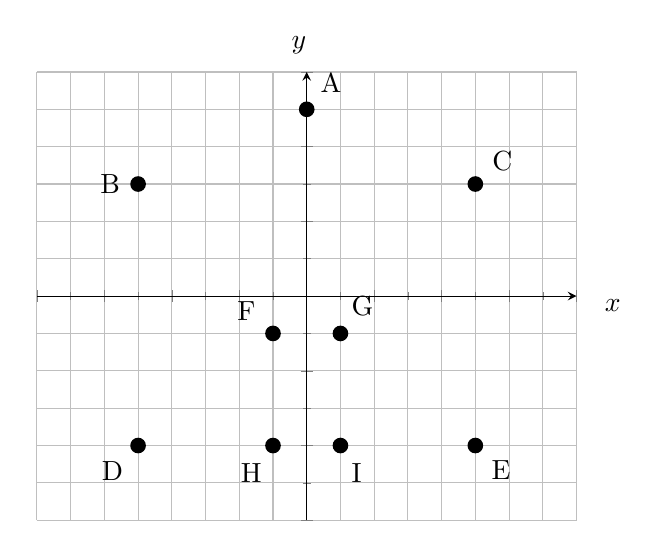
\begin{tikzpicture}
    \begin{axis}[grid=both,ymin=-6,ymax=6,xmax=8,xmin=-8,xticklabel=\empty,yticklabel=\empty,
               minor tick num=1,axis lines = middle,xlabel=$x$,ylabel=$y$,
               label style = {at={(ticklabel cs:1.1)}}]
      \node[label={60:{A}},circle,fill,inner sep=2pt] at (axis cs:0,5) {};
      \node[label={180:{B}},circle,fill,inner sep=2pt] at (axis cs:-5,3) {};
      \node[label={30:{C}},circle,fill,inner sep=2pt] at (axis cs:5,3) {};
      \node[label={230:{D}},circle,fill,inner sep=2pt] at (axis cs:-5,-4) {};
      \node[label={320:{E}},circle,fill,inner sep=2pt] at (axis cs:5,-4) {};
      \node[label={160:{F}},circle,fill,inner sep=2pt] at (axis cs:-1,-1) {};
      \node[label={80:{G}},circle,fill,inner sep=2pt] at (axis cs:1,-1) {};
      \node[label={260:{H}},circle,fill,inner sep=2pt] at (axis cs:-1,-4) {};
      \node[label={280:{I}},circle,fill,inner sep=2pt] at (axis cs:1,-4) {};
    \end{axis}
  \end{tikzpicture}

  \begin{parts}
    \part Busca los puntos en el plano cartesiano.
    \part Ubica coordenadas.
    \part Marca cuadrantes.
    \part Sacar la distancia entre los puntos.
    \part Calcula el perímetro de la figura resultante.
  \end{parts}
